\chapter{Training Convolutional Neural Networks on particles \textcolor{red}{\textbf{WORKING TITLE}}}\label{ch:cnn_train}
Three Convolutional Neural Networks (CNNs) were trained throughout this analysis. There are differences to each CNN and will be described fully in the next sections but the main difference are the amount of particle images used for training and validation. CNN1075 used 1,075 muons and 1,075 pions for training and the same amout of each particle for validation. CNN10000 used 10,000 muons and 10,000 pions split in half for testing and training. Lastly CNN100000 had muons, pions, protons, electrons, and gammas in it's training and validation set. Each particle had 20,000 images and training and validation was split $90\%$ training, $10\%$ validation. This chapter will also describe the different hardware frameworks used for training beginning on a CPU and ending on a GPU cluster.  


\section{Hardware Frameworks used for Training}
\subsection{Syracuse CPU Machine setup}
\subsection{Syracuse University GPU Cluster Setup}


\section{Convolutional Neural Network Training}\label{research approach}

\subsection{Image Making Scheme}\label{image_making} 
\subsubsection{Images used for Traing/Validation of Convolutional Neural Networks}
The $\mu/\pi$ image dataset used to train and validate CNN1075 was created using single generated isotropic muons and poins from 0-2 GeV energy range. 2,150 muons and 2,150 pions were used for training and testing split 50 \%. The images were created based on wire number and time tick in the collection plane. Uboonecode reconstruction version v05{\_}08{\_}00 was used. The raw ADC value after noise filtering was the wire signal. Each collection plane grayscale image was 3456x1600x1 where 6 time ticks were pooled into 1 bin. After the image was created, the region of interest (ROI) in the image was found by using Open CV, a image processing open source software package, to scan the image starting from the edges and stopping once a bright spot is encountered. Thi  

The $\mu/\pi$ image dataset used to train and validate the CNN10000 was also created using single generated isotropic muons and pions from 0-2 GeV energy range. 10,000 muons and 10,000 pions were used for training and testing split 50\%. Uboonecode v06{\_}23{\_}00 was used instead of v05{\_}08{\_}00. Each collection plane grayscale image was 3456x1280x1 where 5 time ticks were pooled into 1 bin which is different than the previous dataset and was implemented due to the fact that the time ticks of an event went from 9400 to 6400 with the change of uboonecode version. The grayscale color standard is 8bit therefore the ADC value of wire and time tick was also downsampled due to the 12bit ADC value MicroBooNE has. To do this, the highest ADC pixel in the image was found and then this was divided by the rest placing all pixel values between 0-1. From there, all pixel values are then multiplied by 255. All images were made using a LArSoft module. Once the images were created, using and image manipulation framework called OpenCV images were read into a numpy array and cropped to the region of interest by only keeping rows and columns where all ADC values are higher than 0 and then resized it to 224x224 using OpenCV's resize function. This downsampling of ADC values creates a problem of information loss for example, a proton which is highly ionizing will have the same brightness as a minimum ionizing muon by virtue of how the images are created. 
Issues that arose in CNN1075 that were fixed in CNN10000 include zero-padding images in X and Y that are smaller than 224X224 to eliminate over-zooming effect and fixing a bug that shifted pixels separated by a dead-wire region. 

Images were also made from events that passed the cc-inclusive selection 1 filter right before the 75 cm track length cut and were classified using the CNN10000. The dataset used to create these images is the same one used in \cite{cc-inclusive}, prodgenie{\_}bnb{\_}nu{\_}cosmic{\_}uboone{\_}mcc7{\_}reco2. These images were created using information from the track candidate that passed the filter. Only wire number and time ticks associated to the track candidate were drawn on the image to mimic a single particle generated image. These images were then classified using CNN10000. Two approaches were taken in making these images. The first was using the image normalization above where the maximum pixel in each image is used as a normalization constant to get all pixels between 0-1 then multiply all pixels by 255. As described above, this is the incorrect way to normalize; it should be normalized by dataset not by event, which is the second way the images were created. The results of CNN10000 performance are shown in section \ref{research approach}. 

\subsection{Training CNN1075}
The work shown in these next sections are based on the previous work done described in \cite{priorwork}. That CNN (now referred to as CNN1075) was trained using single generated isotropic muons and pions from 0-2 GeV energy range. 1,075 muons and pions were used to train the network and 1,075 $\mu/\pi$ were used as a validation set. The accuracy is how well CNN1075 is doing by epoch and was 74.5\%. The loss is gradient descent or minimization of the error of the weights and biases used in each neuron of each layer of CNN1075 and was 58\% with a trend sloping downwards on the loss curve as well as a trend sloping upward in the accuracy curve. Due to the depth of the neural network framework, it was necessary to train with a larger dataset and for more epochs, however, the downward slope of the loss curve is an indication that once trained for longer with a higher training sample, neural networks can be used for $\mu/\pi$ separation. Updates in the image making and downsampling algorithm were made to fix issues that arose in CNN1075. 
\subsection{Training CNN10000}
The hyperparameters used for CNN10000 are shown. The batch size for the training and testing as well as the test iter were chosen to encompass the whole training/testing image set when doing accuracy/loss calculations. To do this, multiplying the test iter by the test batch size give you the amount of images used when calculating accuracy/loss curves. For reference, the accuracy and loss are defined as well. 


\begin{itemize}
 \item \verb|train_batch_size: 100|
 \item \verb|test_batch_size: 100|
 \item \verb|test_iter: 100|
 \item \verb|test_interval: 100|
 \item \verb|base_lr: 0.001|
 \item \verb|lr_policy: "step"|
 \item \verb|gamma: 0.1|
 \item \verb|stepsize: 1000|
 \item \verb|display: 100|
 \item \verb|max_iter: 10000|
 \item \verb|momentum: 0.99|
 \item \verb|weight_decay: 0.0005|
 \item \verb|snapshot: 100|
\item Accuracy: How often the CNN predicts the truth over total number of images
\item Loss: Error between truth and prediction. Minimize loss by gradient descent to update weights and biases of CNN
\end{itemize}

The same architecure that was used to train CNN1075 was employed on CNN10000, Imagenet. Caffe \cite{caffe} was the software package used for both CNNs. The differences include batch size and test{\_}iter and momentum to account for the larger dataset. Both CNNs were trained on a CPU machine, Syracuse01. Further training will be done on a GPU cluster stationed at Syracuse University. Figure \ref{fig:loss_accuracy} shows the loss and accuracy of CNN10000. There is around a 10\% increase in accuracy from CNN1075 to CNN10000, 85\%, and around a 20\% decrease in loss, 36\%.      

\begin{figure}[htp!]
\centering
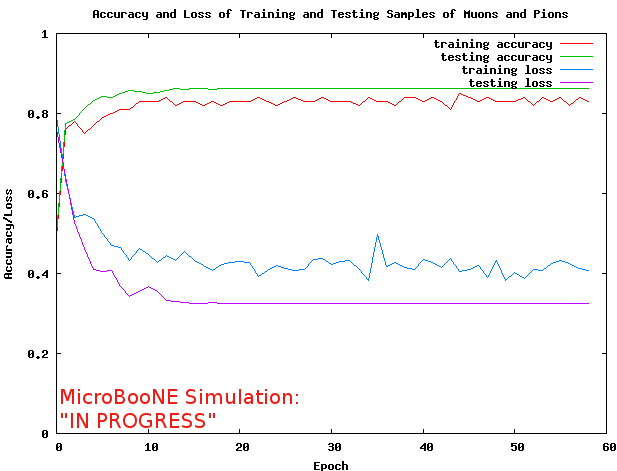
\includegraphics[scale=.4]{figs/acc_loss_10000_062117.png}
\caption{Accuracy vs. Loss of ImageNet 2-output $\mu/\pi$ sample consisting of ~10000 images each.} 
\label{fig:loss_accuracy}
\end{figure}

\begin{figure}[htp!]
\centering
	\begin{subfigure}[b]{.45\textwidth}
	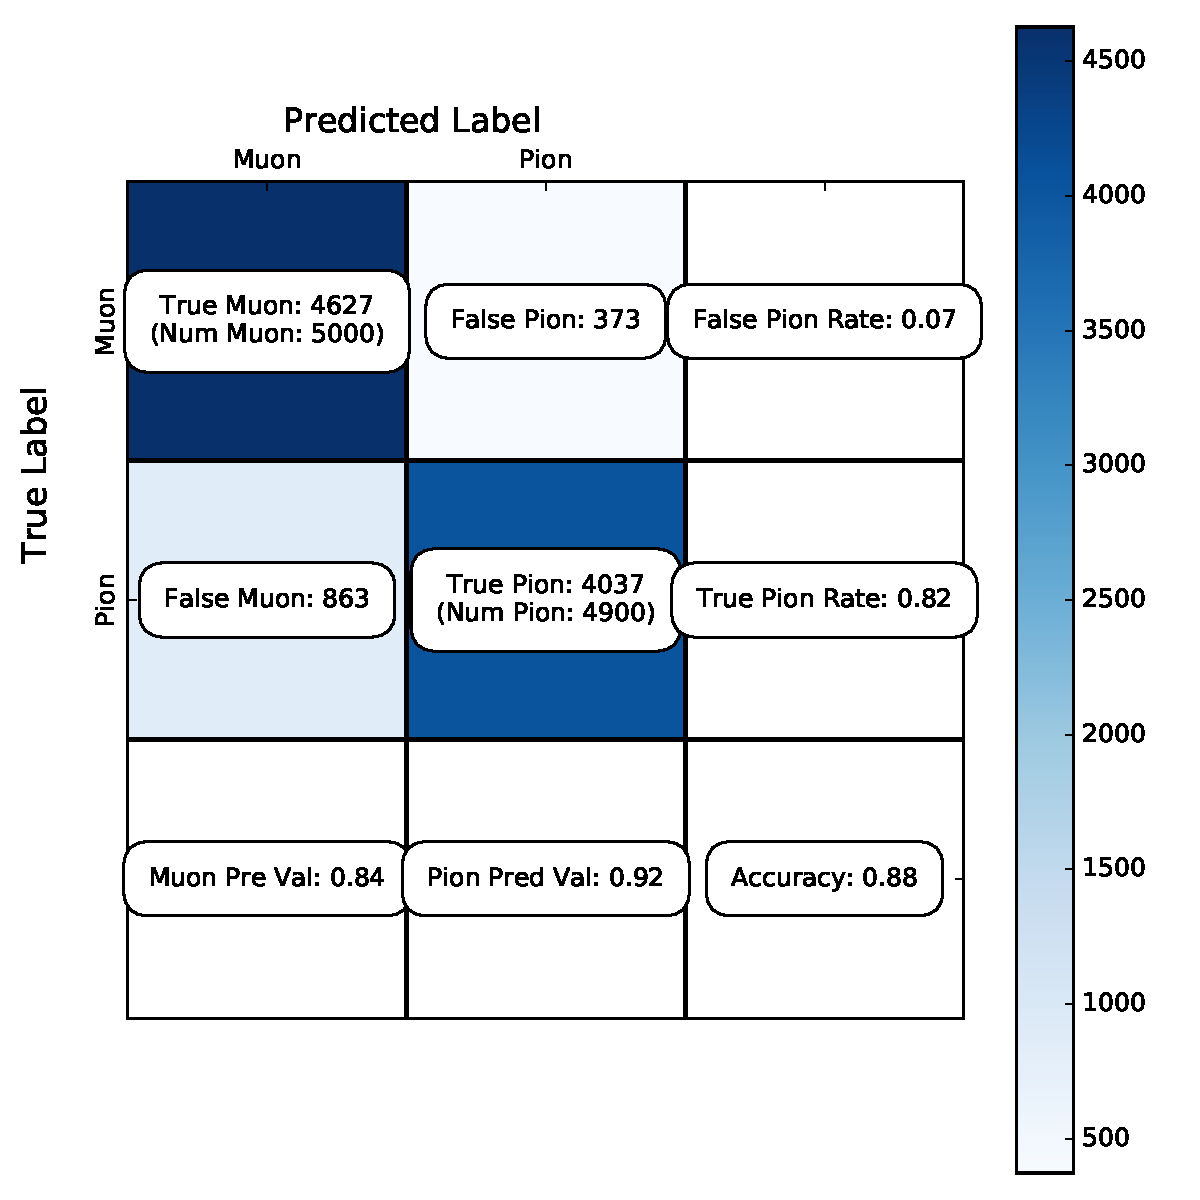
\includegraphics[width=\textwidth,height=3in]{figs/train_confusion.pdf}
	\caption{Confusion Matrix showing Accuracy of CNN using training data}
	\label{fig:confusion}
	\end{subfigure}
	\quad
	\begin{subfigure}[b]{.45\textwidth}
	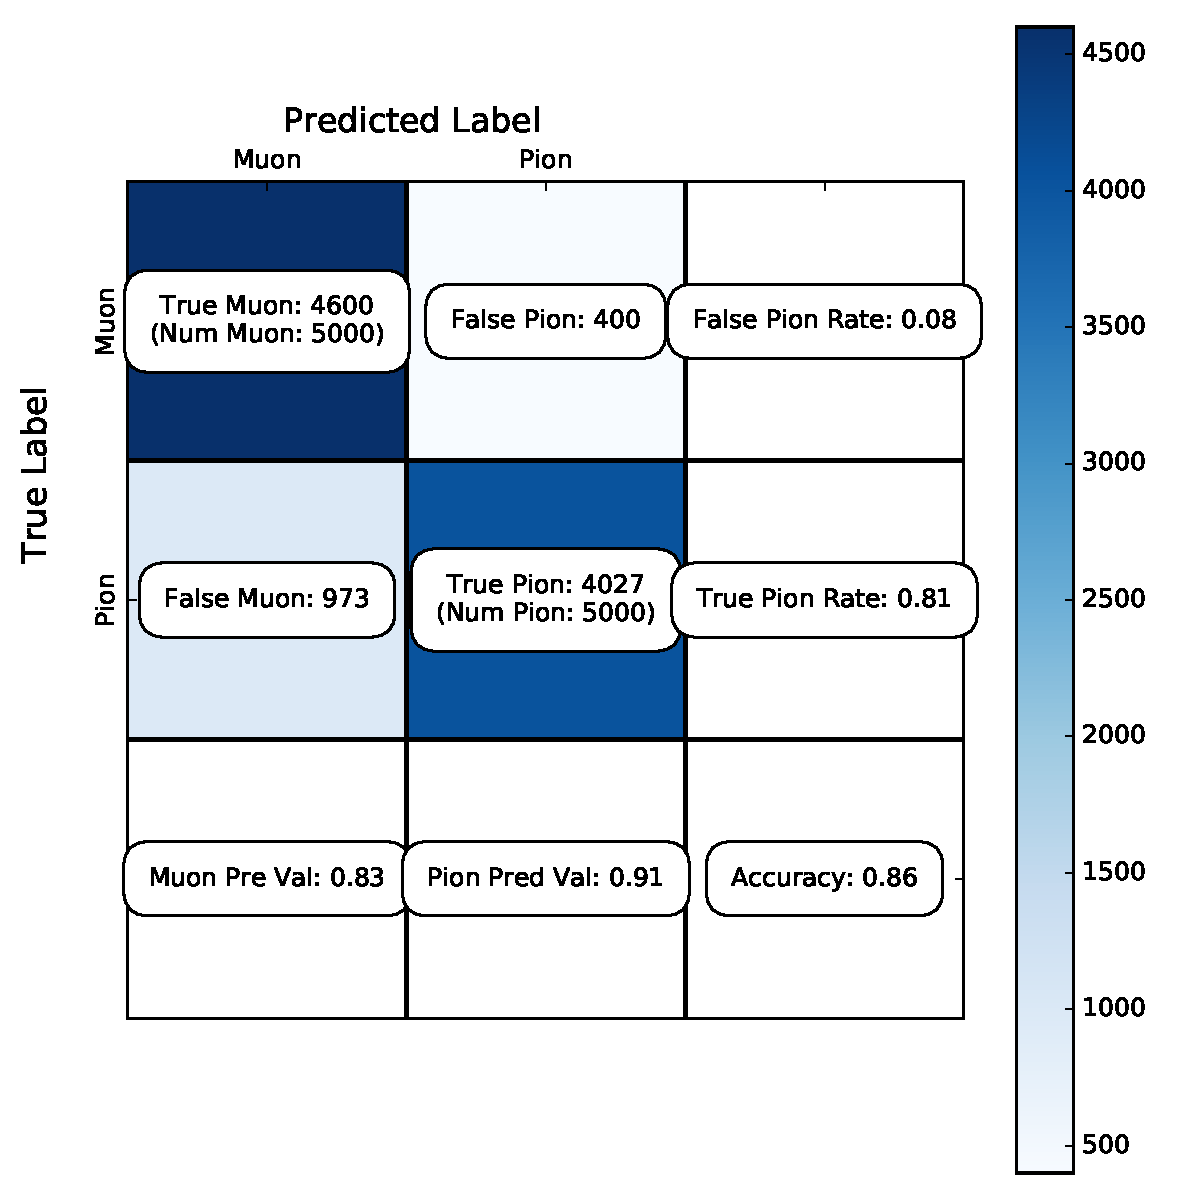
\includegraphics[width=\textwidth,height=3in]{figs/val_confusion.pdf}
	\caption{Confusion Matrix showing Accuracy of CNN using testing data}
	\label{fig:confusion_test}
	\end{subfigure}
	\quad
	\begin{subfigure}[b]{\textwidth}
	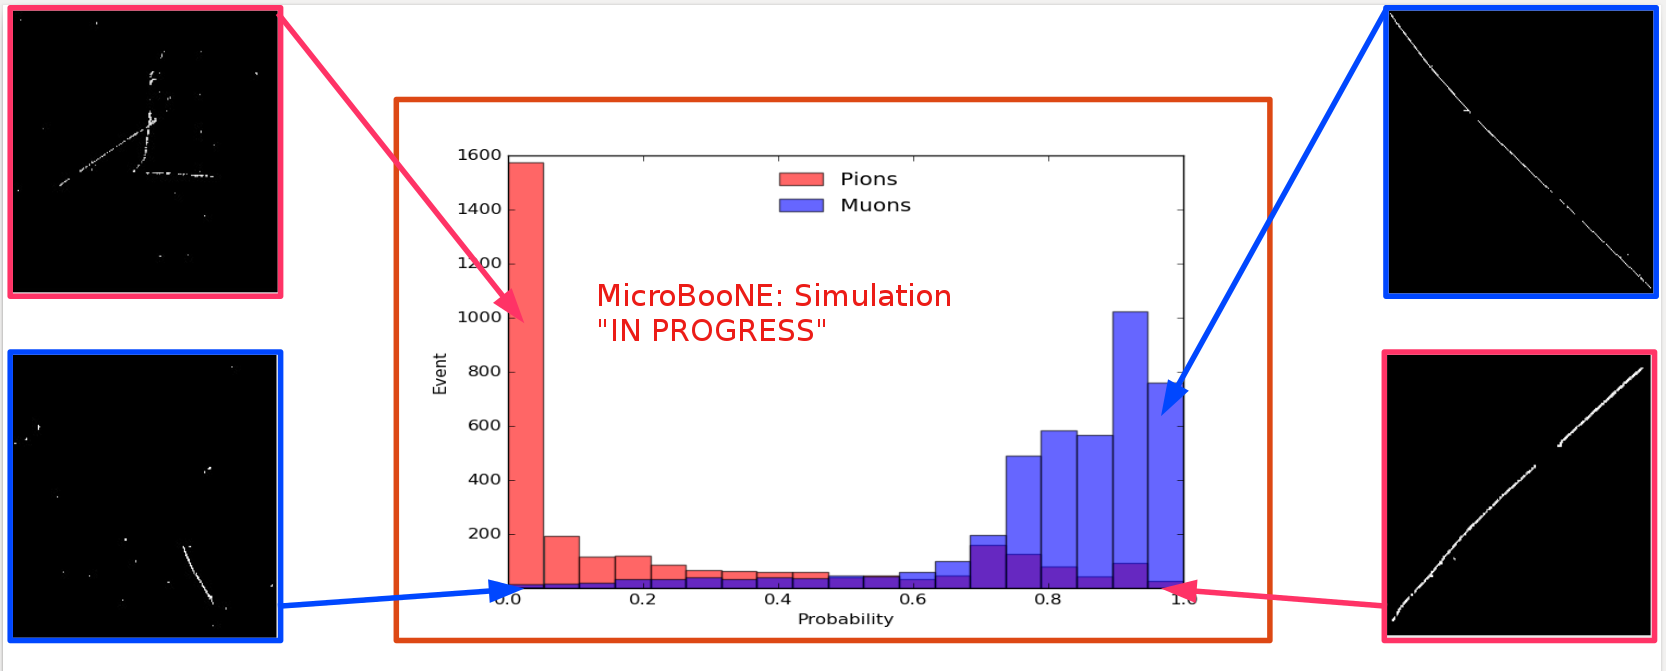
\includegraphics[width=\textwidth,height=2.5in]{figs/mitch_hw.png}
	\caption{Probability plot of muons and pions from testing set. Images surrounding histogram are a random event from lowest bin and highest bin for each particle.}
	\label{fig:prob_plot}
	\end{subfigure}
\caption{Description of confusion matrix varables: False pion rate = $false \pi/ total \pi$ True pion rate = $true \pi/total \pi$ Accuracy = $(true \pi rate + true \mu rate)/2$ Pion prediction value = $true \pi/(true \pi + false \pi)$ Muon prediction value = $true \mu/(true \mu + false \mu)$ \ref{fig:prob_plot} The probability plot includes muons and pions that are classified as primary particles.}
\label{fig:CNN_train}
\end{figure}

Figure \ref{fig:CNN_train} show a breakdown of $\mu/\pi$ separation for CNN10000. It also shows the network is not being overtrained due to the Accuracy of both the training and testing datasets being within .01\% of eachother. The CNN is doing a very good job of classifying true muons as muons, and our loss increase from CNN1075 is due to the increase in accurately classifing pions as pions. 


%\begin{figure}[htp]
%\centering
%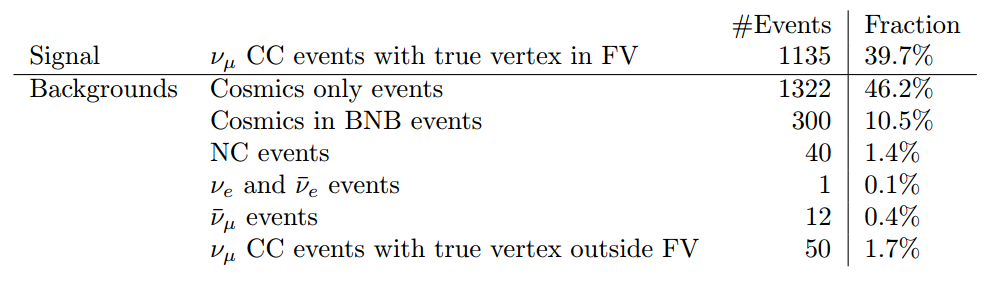
\includegraphics[width=.9\linewidth]{Purity_numbers.png}
%\caption{ Signal and background event numbers at final selection level estimated from a BNB+Cosmic sample and Cosmic only sample normalized to $5*10^{19}$ POT. The last column gives the fraction of this signal or background type to the total 2604 selected events.} 
%\label{fig:puritytable}
%\end{figure}

\subsection{Training CNN100000}
Results of training using 100,000 images, 20,000 images per \mu/\pi/p/\gamma/e. 


\begin{figure}[htp]
\centering
\includegraphics[width=\linewidth=]{../images/confusion_allparticle_v3.pdf}
\caption{Confusion Matrix of all five particles }
\label{fig:confusion100000}
\end{figure}

\begin{figure}[htp]
\centering
\includegraphics[width=.8\linewidth=]{../images/GPU_9010split_hires_iterations_alldata_allparticle.png}
\caption{Training and testing accuracy of CNN trained on 100,000 images of \mu/\pi/p/\gamma/e with 20,000 images of each particle. Each image was a size of 576x576 and the images per particle were split 90\% use for training and 10\% used for testing the network}
\label{fig:gpuacc}
\end{figure}

\begin{figure}[htp]
\centering
\includegraphics[width=.8\linewidth=]{../images/GPU_9010split_hires_iterations_alldata_allparticle_loss.png}
\caption{Training and testing loss oc CNN trained on 100,000 images of \mu/\pi/p/\gamma/e}
\label{fig:gpuloss}
\end{figure}

\begin{figure}[htp]
\centering
\includegraphics[width=.8\linewidth=]{../csv_output/true_labels_1102.png}
\caption{t-SNE of CNN}
\label{fig:tsne}
\end{figure}

\begin{figure}[htp]
\centering
\includegraphics[width=.8\linewidth=]{../csv_output/muon_prob.png}
\caption{Muon Prob}
\label{fig:muonprob}
\end{figure}

\begin{figure}[htp]
\centering
\includegraphics[width=.8\linewidth=]{../csv_output/pi_prob.png}
\caption{Pion Prob}
\label{fig:piprob}
\end{figure}

\begin{figure}[htp]
\centering
\includegraphics[width=.8\linewidth=]{../csv_output/proton_prob.png}
\caption{Proton Prob}
\label{fig:protonprob}
\end{figure}

\begin{figure}[htp]
\centering
\includegraphics[width=.8\linewidth=]{../csv_output/eminus_prob.png}
\caption{Electron Prob}
\label{fig:eminusprob}
\end{figure}

\begin{figure}[htp]
\centering
\includegraphics[width=.8\linewidth=]{../csv_output/gamma_prob.png}
\caption{Gamma Prob}
\label{fig:gammaprob}
\end{figure}

\begin{figure}[htp]
\centering
\includegraphics[width=.8\linewidth=]{../csv_output/prob_allparticle_normalized.pdf}
\caption{Prob}
\label{fig:prob}
\end{figure}

\begin{figure}[htp]
\centering
\includegraphics[width=.8\linewidth=]{../csv_output/mu_pi_acc_tracklength_all.pdf}
\caption{mupi}
\label{fig:mu_pi}
\end{figure}

\begin{figure}[htp]
\centering
\includegraphics[width=.8\linewidth=]{../csv_output/mu_pi_acc_tracklength_75.pdf}
\caption{mupi}
\label{fig:mu_pi}
\end{figure}

\begin{figure}[htp]
\centering
\includegraphics[width=.8\linewidth=]{../csv_output/mu_pi_acc_momentum.pdf}
\caption{mupi}
\label{fig:mu_pi}
\end{figure}

\begin{figure}[htp]
\centering
\includegraphics[width=.8\linewidth=]{../csv_output/mu_p_acc_tracklength_all.pdf}
\caption{mup}
\label{fig:mu_p}
\end{figure}

\begin{figure}[htp]
\centering
\includegraphics[width=.8\linewidth=]{../csv_output/mu_p_acc_tracklength_75.pdf}
\caption{mup}
\label{fig:mu_p}
\end{figure}

\begin{figure}[htp]
\centering
\includegraphics[width=.8\linewidth=]{../csv_output/mu_p_acc_momentum.pdf}
\caption{mup}
\label{fig:mu_p}
\end{figure}

\begin{figure}[htp]
\centering
\includegraphics[width=.8\linewidth=]{../csv_output/mu_e_acc_tracklength_all.pdf}
\caption{mue}
\label{fig:mu_e}
\end{figure}

\begin{figure}[htp]
\centering
\includegraphics[width=.8\linewidth=]{../csv_output/mu_e_acc_tracklength_75.pdf}
\caption{mue}
\label{fig:mu_e}
\end{figure}

\begin{figure}[htp]
\centering
\includegraphics[width=.8\linewidth=]{../csv_output/mu_e_acc_momentum.pdf}
\caption{mue}
\label{fig:mu_e}
\end{figure}

\begin{figure}[htp]
\centering
\includegraphics[width=.8\linewidth=]{../csv_output/mu_g_acc_tracklength_all.pdf}
\caption{mug}
\label{fig:mu_g}
\end{figure}

\begin{figure}[htp]
\centering
\includegraphics[width=.8\linewidth=]{../csv_output/mu_g_acc_tracklength_75.pdf}
\caption{mug}
\label{fig:mu_g}
\end{figure}

\begin{figure}[htp]
\centering
\includegraphics[width=.8\linewidth=]{../csv_output/mu_g_acc_momentum.pdf}
\caption{mug}
\label{fig:mu_g}
\end{figure}

